\documentclass[10pt,twocolumn,a4paper]{article}
\usepackage[margin=18mm,columnsep=7mm]{geometry}
\usepackage[T1]{fontenc}
\usepackage{lmodern}
\usepackage{amsmath,amssymb}
\usepackage{graphicx}
\usepackage{booktabs}
\usepackage{caption}
\usepackage[hidelinks]{hyperref}
\captionsetup{font=small,labelfont=bf}
\setlength{\emergencystretch}{2em}
\graphicspath{{../figures/}}

\newcommand{\ket}[1]{\lvert #1\rangle}
\newcommand{\bra}[1]{\langle #1\rvert}
\newcommand{\proj}[1]{\ket{#1}\!\bra{#1}}
\DeclareMathOperator*{\argmax}{arg\,max}
\DeclareMathOperator{\round}{round}
\newcommand{\Eex}{E_{\mathrm{exact}}}

\title{Drawing the Mona Lisa with Quantum Supersampling}
\author{Rintaro Kanaji (6914500223)\thanks{Homework report for \emph{Programming Quantum
Computers}, Chapter~11.}}
\date{}

\begin{document}
\maketitle

\begin{abstract}
I apply Quantum Supersampling (QSS), introduced in Chapter~11 of
\emph{Programming Quantum Computers}, to a photograph of the Mona Lisa.
The painting is resized to $512\times512$ subpixels, dithered to one bit and
split into $128\times128$ tiles of $4\times4$ subpixels.
Each tile is drawn into the phases of a four-qubit register by a phase oracle.
Its brightness is then estimated by quantum sum estimation, that is, controlled
Grover iterations followed by an inverse quantum Fourier transform (QFT).
I build all circuits at the gate level in Qiskit, derive a closed form for the
QSS lookup table, and find that it agrees with the simulation to within
$10^{-11}$.
I compare QSS with Monte Carlo supersampling at the same number of
shader calls.
With four counter qubits and a single readout per tile, the setting of the
book's lookup-table example, QSS lowers the mean pixel error by $21\%$ and
almost doubles the fraction of exactly correct pixels ($50.8\%$ versus
$28.6\%$).
QSS concentrates its error into fewer but larger, isolated mistakes, which
reproduces the book's main observation that a QPU can change the
\emph{character} of sampling noise.
\end{abstract}

%-------------------------------------------------------------------------
\section{Introduction}

In ray tracing, each output pixel is the average of many samples (rays), a
procedure called \emph{supersampling} or Monte Carlo sampling.
Only the \emph{sum} of the samples is needed, not the samples themselves.
Chapter~11 of the textbook~\cite{pqc} observes that a QPU can estimate such a
sum directly. It combines three primitives for this purpose: quantum
arithmetic (Ch.~5), amplitude amplification (Ch.~6) and the QFT (Ch.~7).
The resulting algorithm, QSS, is not faster than Monte Carlo sampling, but its
error is distributed differently: most pixels come out exact, and a few are
badly wrong.

Throughout, the \emph{shader} is the function $f(x)\in\{0,1\}$ that returns the
value of subpixel $x$. On a QPU the shader is applied as a phase oracle, and the
cost of every method is counted in \emph{shader calls}.
The book demonstrates QSS on synthetic shapes such as lines, circles and
circular bands, whose shaders are short arithmetic circuits.
This report applies the same pipeline to a photograph, which needs a
lookup-table shader instead.
Section~\ref{sec:methods} summarises the methods I use.
Sections~\ref{sec:prep}--\ref{sec:qse} apply them to the image and derive the
readout statistics. Section~\ref{sec:impl} describes the implementation and
its verification, and Sections~\ref{sec:results}--\ref{sec:disc} present and
discuss the results.

%-------------------------------------------------------------------------
\section{Methods}\label{sec:methods}

This section introduces each building block in general form.
Table~\ref{tab:methods} lists where each one comes from and what role it
plays in this work.

\begin{table}[t]
\centering\footnotesize
\setlength{\tabcolsep}{3pt}
\caption{Methods used in this work.}
\label{tab:methods}
\begin{tabular}{lll}
\toprule
Method & Source & Role here\\
\midrule
Superposition (H gates) & Ch.~2 & blank canvas $\ket{s}$\\
Phase encoding / oracle & Ch.~4, 11 & draw one tile\\
Amplitude amplification & Ch.~6 & Grover iteration $Q$\\
QFT / phase estimation & Ch.~7 & read the counter\\
Quantum sum estimation & Ch.~6, 11 & count white pixels\\
QSS lookup table & Ch.~11 & readout $\to$ brightness\\
Bayer dithering & classical & grey $\to$ 1 bit\\
Bitplanes & Ch.~11 & colour\\
Monte Carlo sampling & classical & baseline\\
\bottomrule
\end{tabular}
\end{table}

\paragraph{Superposition and phase encoding.}
Hadamard gates on an $n$-qubit register give the uniform superposition
$\ket{s}=2^{-n/2}\sum_x\ket{x}$, in which every basis state stands for one
pixel. A Boolean function $f$ is written into the state by the phase oracle
$O_f\ket{x}=(-1)^{f(x)}\ket{x}$. A single phase flip of a basis state
$\ket{x_0}$ is implemented by a multi-controlled $Z$ gate, with $X$ gates on the
qubits where $x_0$ has a $0$.

\paragraph{Amplitude amplification.}
The Grover iteration $Q=(I-2\proj{s})\,O_f$ consists of the oracle followed
by a reflection about $\ket{s}$, the book's \texttt{mirror}. If a fraction
$a=\sin^2\theta$ of the basis states is marked, then $Q$ rotates the state by
$2\theta$ in the plane spanned by the marked and unmarked states. After $m$
iterations the probability of a marked state is $\sin^2((2m+1)\theta)$. This
probability oscillates in $m$ with a frequency set by $a$.

\paragraph{QFT and phase estimation.}
The QFT maps $\ket{y}\mapsto N^{-1/2}\sum_m e^{2\pi i\,my/N}\ket{m}$, and its
inverse turns a phase that grows linearly in $m$ into a peak at the
corresponding frequency. Controlling $U^{2^j}$ with the $j$-th qubit of a
counter register and then applying $\mathrm{QFT}^\dagger$ estimates an
eigenphase of $U$ with resolution $1/N$, where $N=2^t$.

\paragraph{Quantum sum estimation.}
Quantum sum estimation is phase estimation applied to $U=Q$. Its readout
reveals $\theta$, and hence the number of marked items $k=16\sin^2\theta$
(the book's ``Multiple Flipped Entries'' example, also known as quantum
counting~\cite{brassard}). QSS uses this to obtain the \emph{sum} over all
subpixels of a tile without reading any single subpixel.

\paragraph{QSS lookup table.}
The readout is related to $k$ only statistically. A table $P(y\mid k)$,
computed once for a given tile size and counter size, converts a readout into
the most likely $k$ and gives a confidence for that value.

\paragraph{Classical components.}
Ordered dithering converts grey levels into one-bit images whose local density
equals the grey level. Bitplanes treat each colour channel as a separate
one-bit image. Monte Carlo sampling estimates a tile's brightness from
randomly chosen subpixels and serves as the baseline.

\paragraph{Tools.}
All circuits are built and simulated with Qiskit~2.6, using exact
statevector simulation. NumPy, SciPy, Pillow and Matplotlib are used for image
processing, statistics and figures.

%-------------------------------------------------------------------------
\section{Image preparation}\label{sec:prep}

The input is a $408\times530$ RGB image.
I crop a $408\times408$ square starting at row~20 so that the head is kept,
then resize it to $512\times512$ with Lanczos filtering.
A $4\times4$ Bayer matrix
\begin{equation}
B=\begin{pmatrix}0&8&2&10\\12&4&14&6\\3&11&1&9\\15&7&13&5\end{pmatrix}
\end{equation}
is aligned with the tile grid. A subpixel of grey level $g\in[0,1]$ at
position $(u,v)$ is set white ($b_{uv}=1$) when
\begin{equation}
g_{uv} \ge \frac{B_{u\bmod 4,\,v\bmod 4}+\tfrac12}{16}.
\end{equation}
Each threshold occurs exactly once per tile, so a tile of uniform grey level
$g$ contains exactly $k=\lfloor 16g+\tfrac12\rfloor$ white subpixels.
The number of white subpixels is therefore a faithful 17-level measure of
brightness, and the \emph{ideal} brightness of output pixel $(i,j)$ is
\begin{equation}
L^{\star}_{ij}=\frac{k_{ij}}{16},\qquad k_{ij}=\sum_{(u,v)\in T_{ij}} b_{uv},
\label{eq:ideal}
\end{equation}
where $T_{ij}$ is the tile in row $i$ and column $j$.
For colour, the R, G and B channels are dithered independently into three
bitplanes. Figure~\ref{fig:prep} shows the stages.

\begin{figure*}[t]
\centering
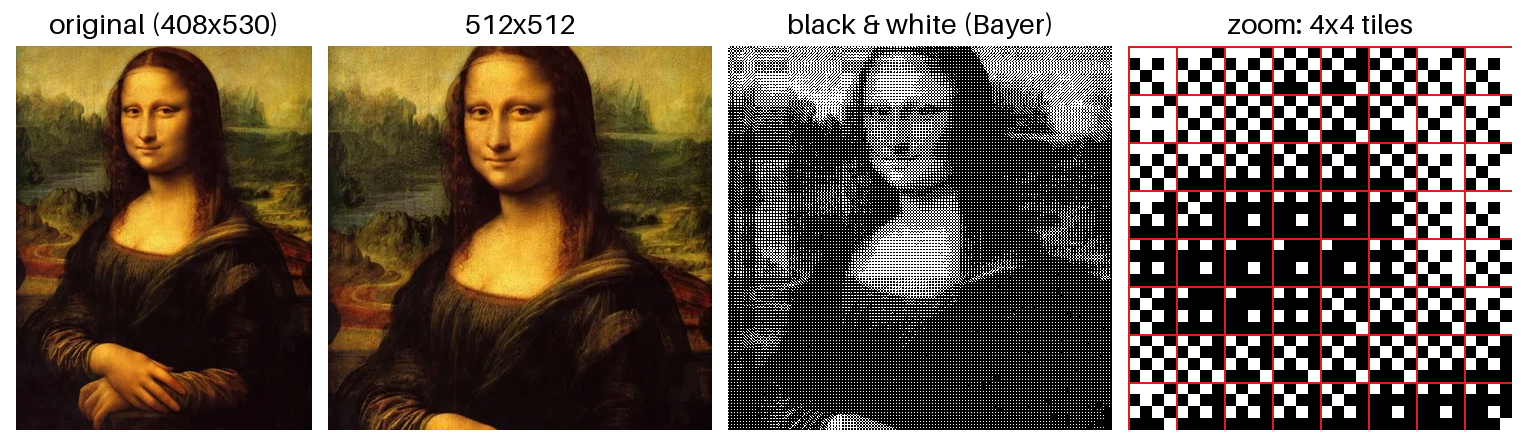
\includegraphics[width=\textwidth]{step1_overview.png}
\caption{Image preparation. From left: original ($408\times530$),
$512\times512$ crop, one-bit Bayer image (white $=$ phase $\pi$), and a
$32\times32$ zoom with the $4\times4$ tile grid in red. Each tile becomes one
output pixel.}
\label{fig:prep}
\end{figure*}

%-------------------------------------------------------------------------
\section{Phase-encoded tiles}\label{sec:encode}

A tile is addressed by two 2-qubit registers $q_x,q_y$, combined into the
4-qubit index $x=4q_y+q_x\in\{0,\dots,15\}$.
The shader $f(x)=b_{uv}$ returns the dithered bit of the subpixel $(u,v)$ of
the tile that has index $x$.
Hadamard gates prepare a blank canvas, and the phase oracle
$O_f\ket{x}=(-1)^{f(x)}\ket{x}$ paints the white subpixels:
\begin{equation}
\begin{split}
\ket{s}&=H^{\otimes4}\ket{0}=\frac14\sum_{x=0}^{15}\ket{x},\\
O_f\ket{s}&=\frac14\sum_{x=0}^{15}(-1)^{f(x)}\ket{x}.
\end{split}
\end{equation}
This is the book's \emph{phase encoding}. All amplitudes have magnitude
$1/4$, and the image is stored only in the signs
(Fig.~\ref{fig:circle}).
A photograph has no compact arithmetic description, so I write the oracle as
a product of single-state phase flips,
\begin{equation}
O_f=\prod_{x:\,f(x)=1}\Bigl(X^{\bar x}\, C^{3}Z\, X^{\bar x}\Bigr),
\label{eq:oracle}
\end{equation}
where $X^{\bar x}$ applies $X$ to every qubit whose bit of $x$ is $0$, and
$C^3Z$ is a Z gate controlled by three qubits, which flips the phase of
$\ket{1111}$.

\begin{figure}[t]
\centering
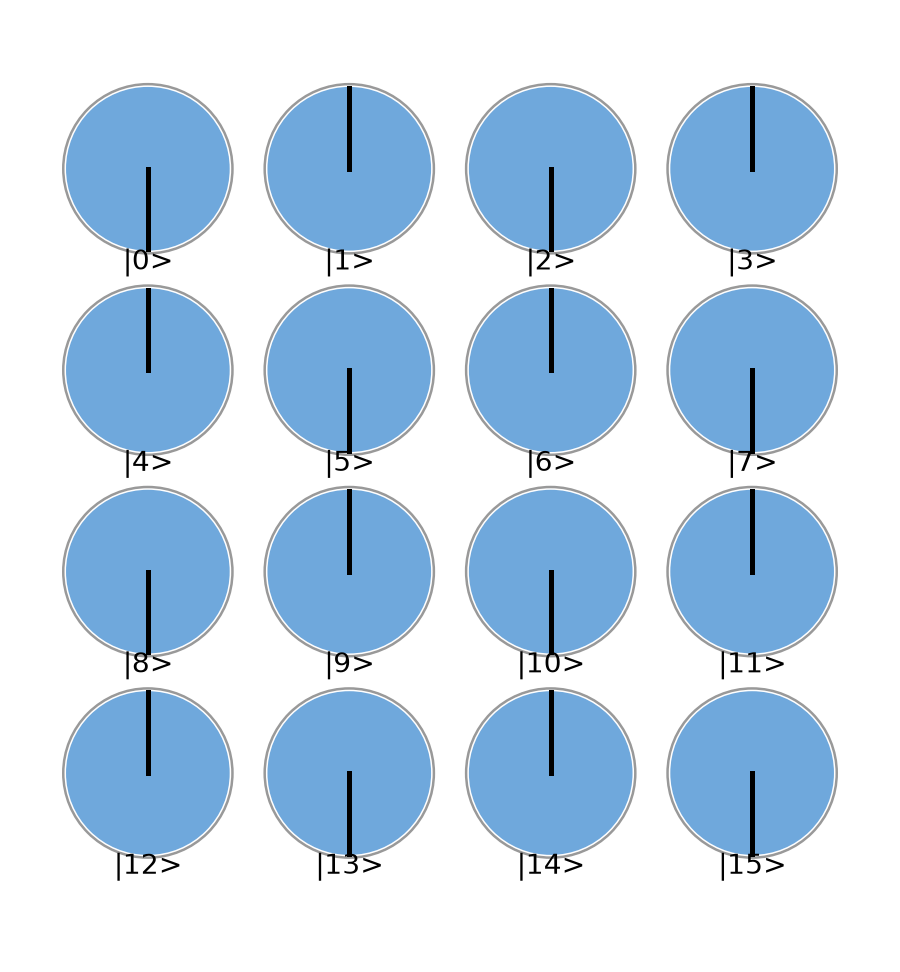
\includegraphics[width=0.62\columnwidth]{circle_notation_tile.png}
\caption{Circle notation of the tile in row~35, column~64 (a checkerboard,
$k=8$) after $H^{\otimes4}$ and $O_f$. A line pointing up means phase $0$
(black); a line pointing down means phase $\pi$ (white).}
\label{fig:circle}
\end{figure}

%-------------------------------------------------------------------------
\section{Quantum sum estimation}\label{sec:qse}

\subsection{Grover iteration}
I use the book's \texttt{grover\_iteration}, which reflects about $\ket{s}$:
\begin{equation}
\begin{split}
Q&=\bigl(I-2\proj{s}\bigr)\,O_f\\
 &=H^{\otimes4}X^{\otimes4}\,C^{3}Z\,X^{\otimes4}H^{\otimes4}\,O_f .
\end{split}
\label{eq:Q}
\end{equation}
Define $\theta\in[0,\pi/2]$ by
\begin{equation}
\sin^2\theta=\frac{k}{16},
\end{equation}
and the normalised states
$\ket{w}=k^{-1/2}\sum_{f(x)=1}\ket{x}$ and
$\ket{b}=(16-k)^{-1/2}\sum_{f(x)=0}\ket{x}$, so that
$\ket{s}=\sin\theta\ket{w}+\cos\theta\ket{b}$.
On the plane spanned by $\ket{b}$ and $\ket{w}$, $O_f$ is a reflection
about $\ket{b}$ and $2\proj{s}-I$ is a reflection about $\ket{s}$, so their
product is a rotation by $2\theta$. Because Eq.~\eqref{eq:Q} carries an
extra minus sign, $Q$ acts in the basis $(\ket{b},\ket{w})$ as
\begin{equation}
Q=-\begin{pmatrix}\cos2\theta&-\sin2\theta\\ \sin2\theta&\cos2\theta\end{pmatrix},
\end{equation}
with eigenvalues $e^{i(\pi\pm2\theta)}$ and eigenvectors $\ket{\psi_\pm}$.
The start state is an equal-weight superposition of the two,
\begin{equation}
\ket{s}=\tfrac{1}{\sqrt2}\bigl(e^{i\alpha}\ket{\psi_+}+e^{-i\alpha}\ket{\psi_-}\bigr),
\label{eq:split}
\end{equation}
where $\alpha$ is a phase that does not affect the measurement
probabilities. (For $k=0$ or $16$ the two eigenvalues coincide and $\ket{s}$
is itself an eigenvector.)

\subsection{Counter register and inverse QFT}
A $t$-qubit counter in uniform superposition controls $Q^{2^j}$ on its
$j$-th qubit, so counter value $m$ triggers exactly $m$ iterations:
\begin{equation}
\frac{1}{\sqrt N}\sum_{m=0}^{N-1}\ket{m}\otimes Q^{m}\ket{s},\qquad N=2^t .
\end{equation}
Applying $\mathrm{QFT}^{\dagger}$ to the counter and measuring gives a
readout $y\in\{0,\dots,N-1\}$. For an eigenphase $2\pi\varphi$ the readout
distribution is the normalised Fej\'er kernel
\begin{equation}
F_N(\delta)=\left|\frac1N\sum_{m=0}^{N-1}e^{2\pi i m\delta}\right|^2
=\frac{\sin^2(\pi N\delta)}{N^2\sin^2(\pi\delta)},
\label{eq:fejer}
\end{equation}
where $\delta=\varphi-y/N$ and $\sum_y F_N=1$. With Eq.~\eqref{eq:split} and
$\varphi_\pm=\tfrac12\pm\theta/\pi$, the \emph{QSS lookup table} has the closed
form
\begin{equation}
\boxed{P(y\mid k)=\tfrac12\Bigl[F_N\!\bigl(\varphi_+-\tfrac yN\bigr)
+F_N\!\bigl(\varphi_- -\tfrac yN\bigr)\Bigr]}
\label{eq:lut}
\end{equation}
for all $0\le k\le16$. Three consequences follow.
(i)~$P(y\mid k)$ depends only on $k$, not on \emph{where} the white subpixels
are.
(ii)~Its peaks sit at
\begin{equation}
y\approx N\Bigl(\tfrac12\pm\tfrac{1}{\pi}\arcsin\sqrt{k/16}\Bigr)\pmod N ,
\end{equation}
so black tiles ($k=0$) are read near $y=N/2$ and white tiles ($k=16$) near
$y=0$.
(iii)~Because $\varphi_++\varphi_-=1$ and $F_N$ is even and 1-periodic,
$P(y\mid k)=P(N-y\mid k)$. The readouts $y$ and $N-y$ carry the same
information, so at most $N/2+1$ distinct values of $k$ can be decoded.

\subsection{Decoding and confidence}
Book Example~11-5 builds the table. As in Example~11-4
(\texttt{qss\_count\_to\_hits}), I decode a readout to the most likely
count,
\begin{equation}
\hat k(y)=\argmax_{k}P(y\mid k),\qquad \hat L_{ij}=\hat k(y_{ij})/16 .
\end{equation}
The confidence of a pixel is the posterior probability of the decoded value
under a uniform prior,
\begin{equation}
c(y)=\frac{P(y\mid\hat k(y))}{\sum_{k=0}^{16}P(y\mid k)} .
\label{eq:conf}
\end{equation}
Figure~\ref{fig:lut} shows the tables. With $t=4$, consequence (iii) leaves
only nine decodable levels, $\hat k\in\{0,1,2,5,8,11,14,15,16\}$. Tiles with
$k\in\{3,4,6,7,9,10,12,13\}$ can never be decoded exactly. With $t=6$ all 17
levels are decodable.

\begin{figure*}[t]
\centering
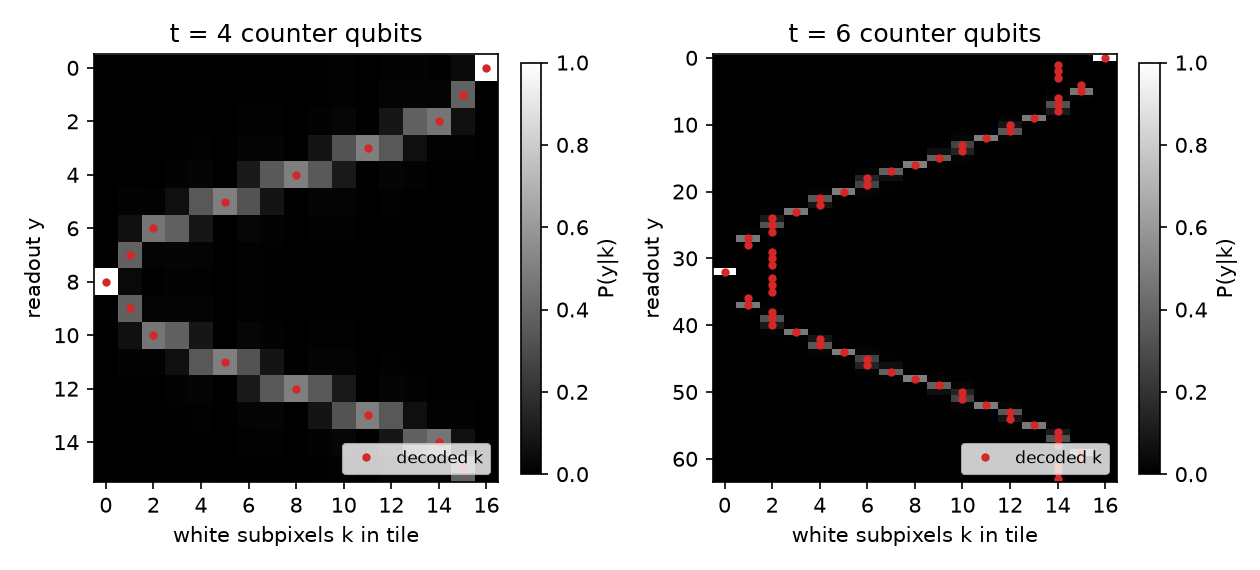
\includegraphics[width=0.7\textwidth]{lookup_tables.png}
\caption{QSS lookup tables $P(y\mid k)$ for $4\times4$ tiles with $t=4$ (left)
and $t=6$ (right) counter qubits. Red dots mark $\hat k(y)$. Each table is
symmetric under $y\leftrightarrow N-y$. With $t=4$ only nine levels are
decodable and neighbouring columns overlap; with $t=6$ every $k$ has its own
peak. Compare book Figs.~11-14 and 11-16.}
\label{fig:lut}
\end{figure*}

\subsection{Circuits}
Figure~\ref{fig:qss} shows the circuit for one tile with $t=4$, which uses
$4+t=8$ qubits.
The controlled iteration needs only \emph{one} extra control on each
$C^3Z$ gate (Fig.~\ref{fig:grover}). When the control is $\ket0$, the $X$ and
$H$ conjugations cancel in pairs. This is the same idea as the book's
\texttt{mask\_with\_condition}.
Figure~\ref{fig:iqft} shows the inverse QFT.
After decomposition into CNOT and single-qubit gates, a $t=4$ tile circuit
contains about $1.6\times10^{3}$ CNOTs and a $t=6$ circuit (10 qubits)
about $6.8\times10^{3}$.

\begin{figure}[t]
\centering
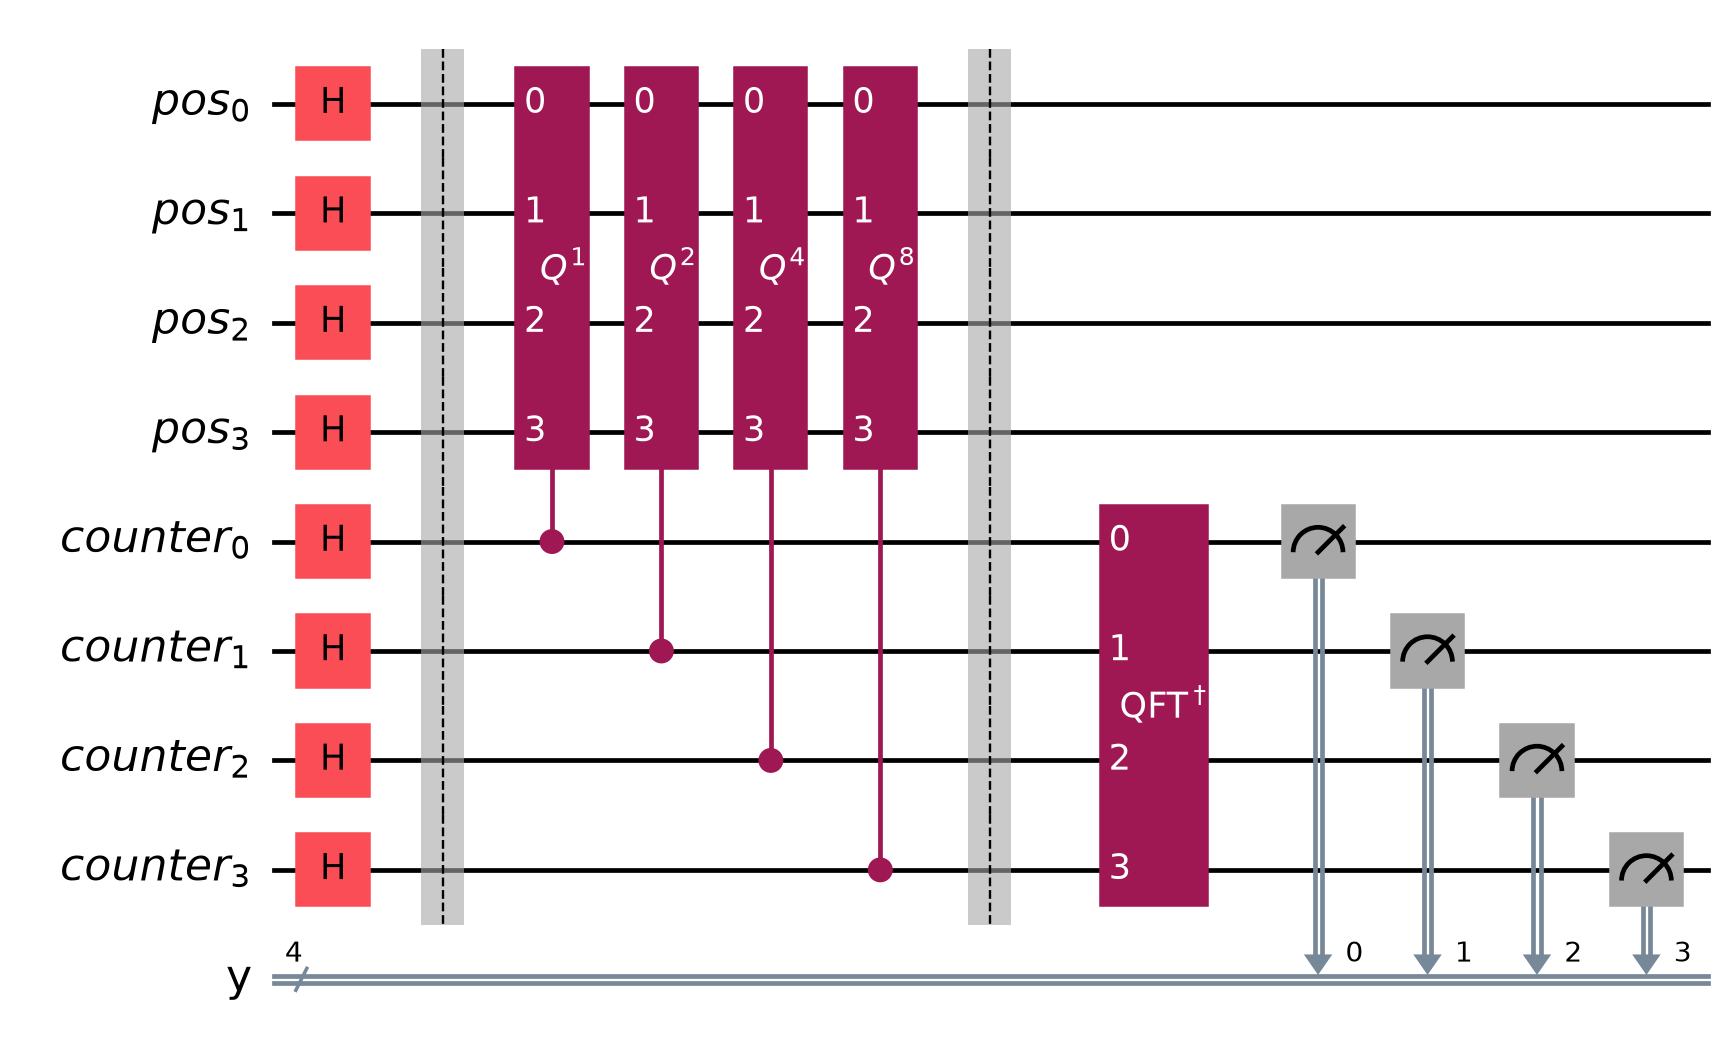
\includegraphics[width=\columnwidth]{circuit_qss_overview_t4.png}
\caption{QSS circuit for one tile ($t=4$). Counter qubit $c_j$ controls
$Q^{2^j}$; $\mathrm{QFT}^\dagger$ converts the counter phases into a readout
$y$.}
\label{fig:qss}
\end{figure}

\begin{figure}[t]
\centering
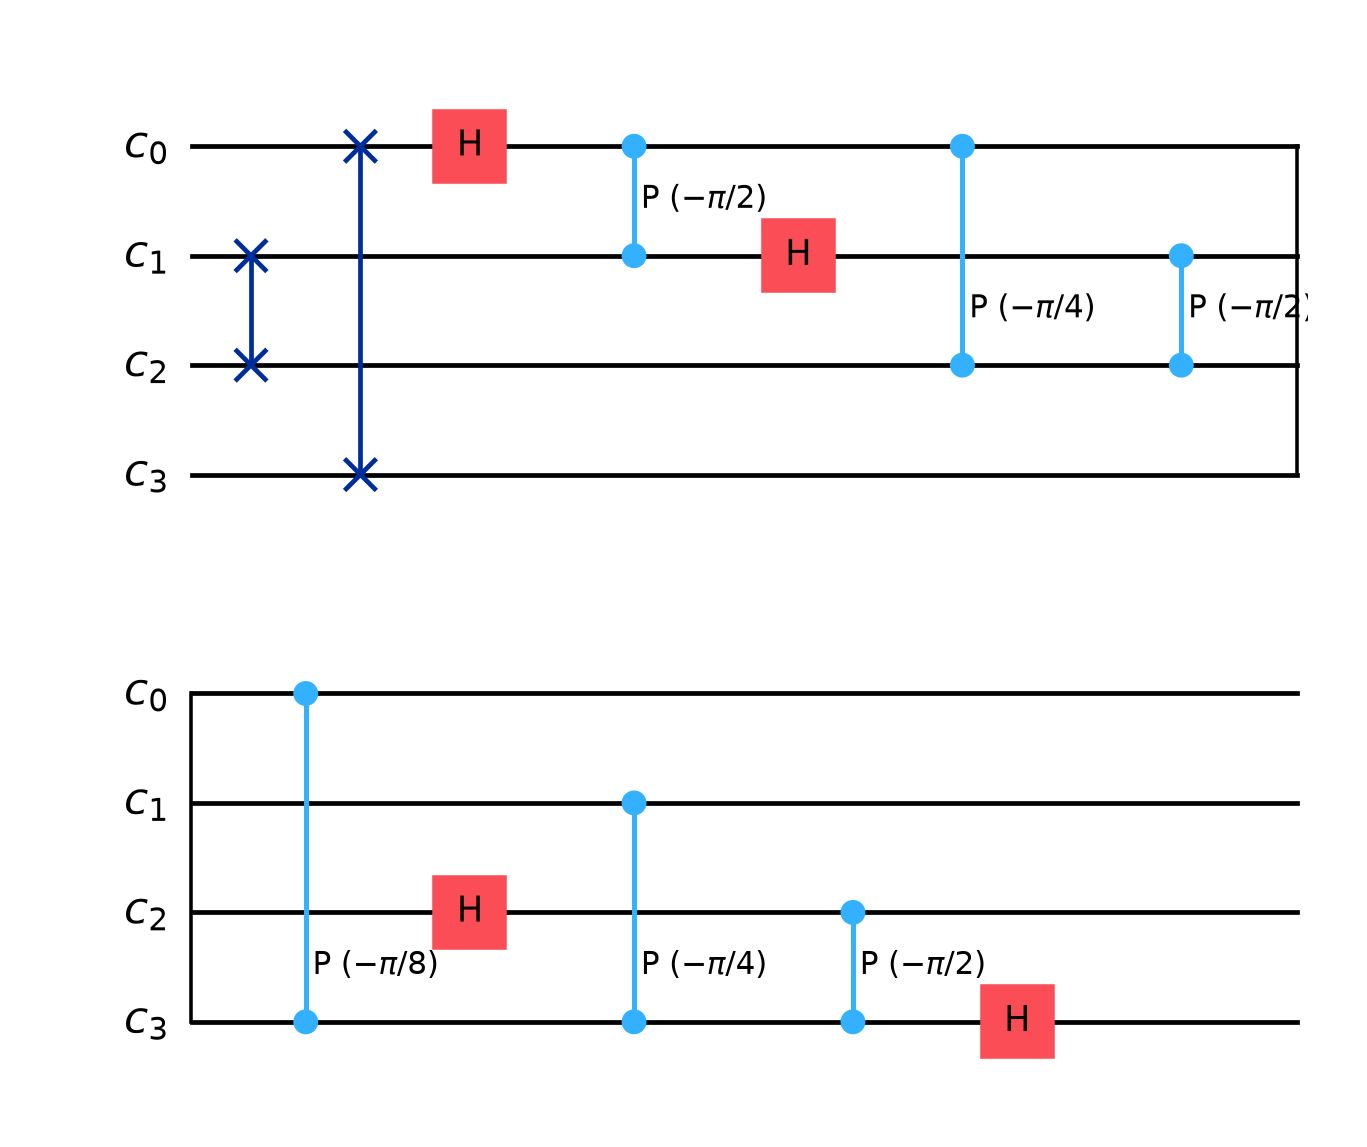
\includegraphics[width=0.85\columnwidth]{circuit_inverse_qft_t4.png}
\caption{Four-qubit inverse QFT on the counter: bit-reversal SWAPs, Hadamards
and controlled phases $P(-\pi/2^{\ell})$.}
\label{fig:iqft}
\end{figure}

\begin{figure*}[t]
\centering
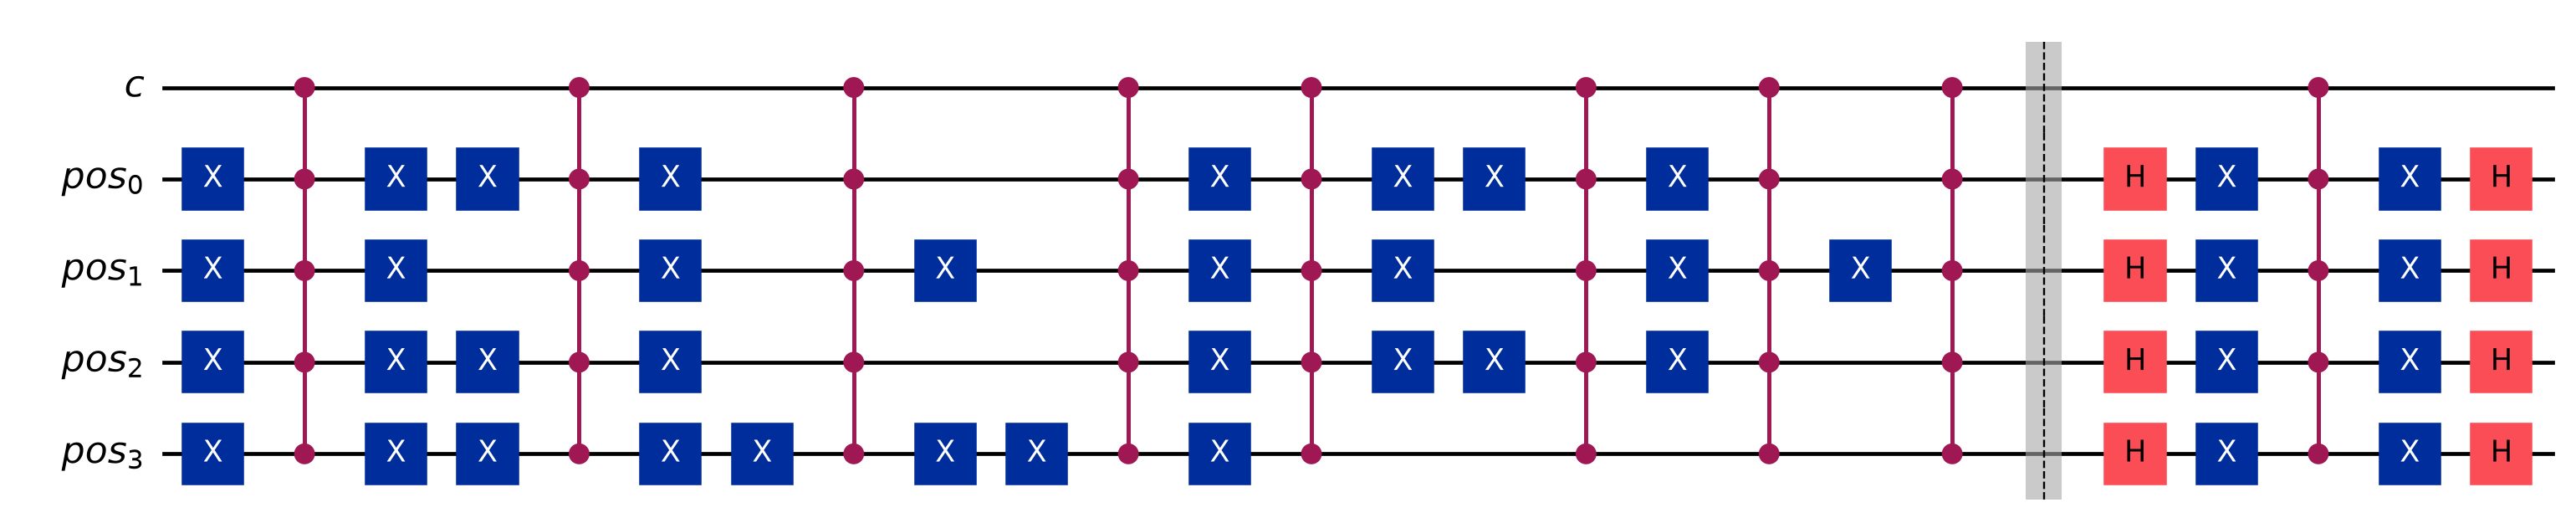
\includegraphics[width=\textwidth]{circuit_grover_step_controlled.png}
\caption{Gate-level controlled-$Q$ for the tile in row~35, column~64.
Left of the barrier: the oracle $O_f$, made of eight phase flips of the form of
Eq.~\eqref{eq:oracle}. Right: the diffusion $I-2\proj{s}$. Only the
multi-controlled $Z$ gates carry the counter control $c$.}
\label{fig:grover}
\end{figure*}

%-------------------------------------------------------------------------
\section{Implementation and verification}\label{sec:impl}

The circuits are built from Qiskit~2.6 gates ($H$, $X$, multi-controlled $Z$,
\texttt{QFTGate}) and simulated exactly with \texttt{Statevector}.
I verified the implementation in four ways (Table~\ref{tab:verify}):
(a)~the unitary of the gate-level $Q$ equals the matrix
$(I-2\proj s)\,\mathrm{diag}((-1)^{f})$;
(b)~for every $k$, a mask with its white subpixels randomly permuted gives
the same $P(y)$;
(c)~40 real tiles of the Mona Lisa give the table column for their own $k$;
(d)~the simulated table equals the closed form, Eq.~\eqref{eq:lut}.

\begin{table}[t]
\centering\small
\setlength{\tabcolsep}{4pt}
\caption{Maximum absolute deviation in each verification test.}
\label{tab:verify}
\begin{tabular}{lcc}
\toprule
Test & $t=4$ & $t=6$\\
\midrule
(a) gate-level $Q$ vs.\ matrix & $4.6\times10^{-15}$ & $1.6\times10^{-15}$\\
(b) permuted masks vs.\ table & $9.3\times10^{-15}$ & $4.0\times10^{-14}$\\
(c) 40 real tiles vs.\ table  & $1.9\times10^{-14}$ & $6.1\times10^{-14}$\\
(d) sim.\ vs.\ closed form & $1.6\times10^{-12}$ & $6.7\times10^{-12}$\\
\bottomrule
\end{tabular}
\end{table}

Tests (b) and (c) show that the readout statistics of a tile are fully
determined by its count $k$.
I therefore render the full image by drawing one readout $y_{ij}$ per tile
from $P(y\mid k_{ij})$.
This is statistically identical to running and measuring each of the
$16\,384$ tile circuits once, and it takes seconds instead of hours.

\begin{figure*}[t]
\centering
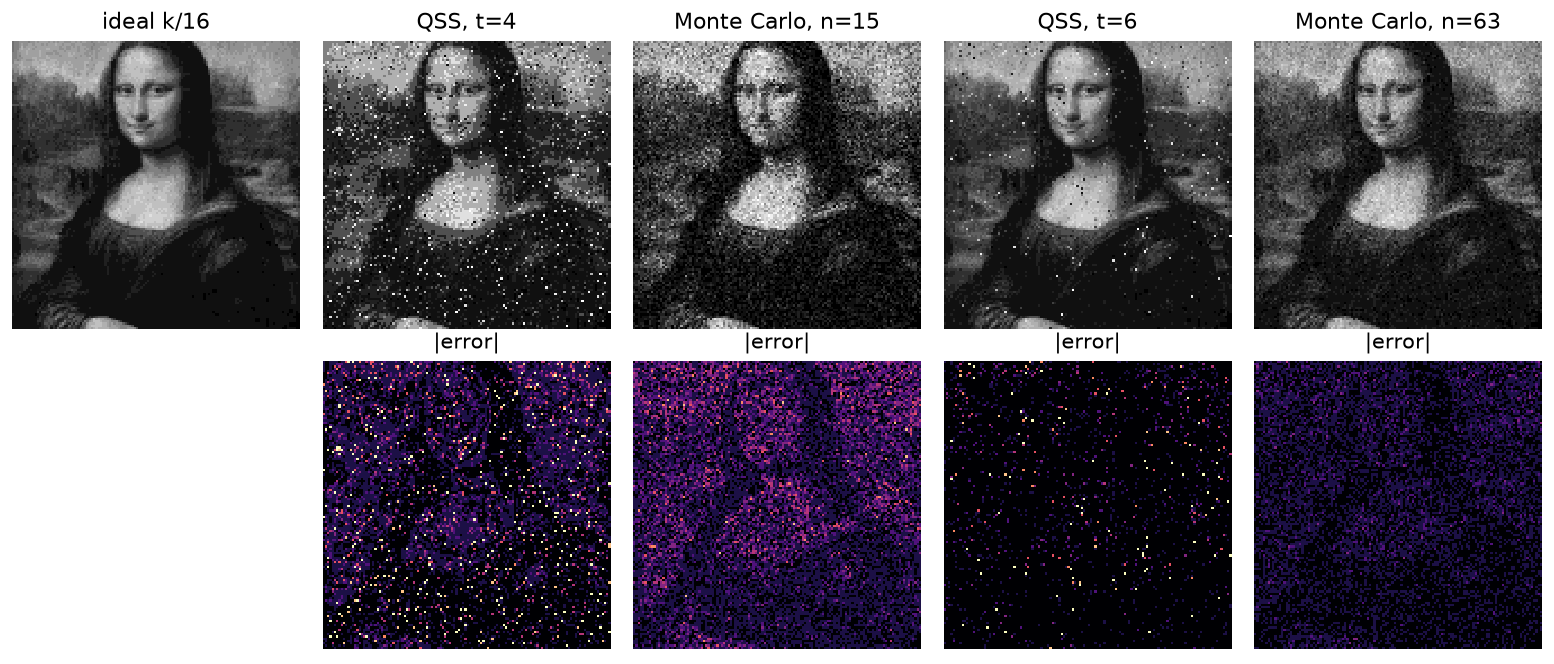
\includegraphics[width=\textwidth]{comparison_gray.png}
\caption{Greyscale results ($128\times128$). Top, from left: ideal
(Eq.~\eqref{eq:ideal}); QSS with $t=4$ and Monte Carlo with $n=15$ shader
calls; QSS with $t=6$ and Monte Carlo with $n=63$. Each QSS tile uses a
single readout. Bottom: absolute error $|\hat L-L^\star|$.}
\label{fig:gray}
\end{figure*}

\subsection{Monte Carlo baseline}
Conventional supersampling evaluates the shader at $n$ subpixels chosen
uniformly at random (with replacement). The number of white hits $h$ follows
$h\sim\mathrm{Bin}(n,k/16)$, and the estimate is
$\tilde L=\round(16h/n)/16$, rounded to the same 17 levels.
The circuit of Fig.~\ref{fig:qss} calls the shader
$\sum_{j=0}^{t-1}2^j=2^t-1$ times, so for equal cost I use $n=2^t-1$,
which is 15 for $t=4$ and 63 for $t=6$. The standard error of the Monte Carlo
estimate of $p=k/16$ is
\begin{equation}
\sigma_{\mathrm{MC}}=\sqrt{\frac{p(1-p)}{n}}=O(n^{-1/2}).
\end{equation}
The QSS peak width in Eq.~\eqref{eq:fejer} is $O(1/N)$ in $\varphi$, and hence
also in $p=\sin^2\theta$. This is the quadratic speed-up of amplitude
estimation~\cite{brassard}.
This baseline models a renderer, where the number of possible samples is
effectively unlimited. A tile here has only 16 subpixels, so 16 deterministic
shader calls would give the exact value classically. The comparison is
therefore at a fixed sample budget, as in the book, and is not the best
possible classical strategy for this toy problem.

%-------------------------------------------------------------------------
\section{Results}\label{sec:results}

For any estimate $\hat L$ (QSS) or $\tilde L$ (Monte Carlo) I report the mean
absolute error
$\mathrm{MAE}=\frac{1}{|\Omega|}\sum_{ij}|\hat L_{ij}-L^{\star}_{ij}|$ and the
fraction of exactly correct pixels
$\Eex=\frac{1}{|\Omega|}\#\{ij:\hat L_{ij}=L^\star_{ij}\}$. Here $\Omega$ is the
set of $128\times128$ pixels. With $w(k)=\#\{ij:k_{ij}=k\}/|\Omega|$, the
fraction of tiles with count $k$, the expected values for QSS are
\begin{align}
\mathbb E[\mathrm{MAE}]&=\sum_{k}w(k)\sum_{y}P(y\mid k)\,\frac{|\hat k(y)-k|}{16},\\
\mathbb E[\Eex]&=\sum_k w(k)\sum_y P(y\mid k)\,[\hat k(y)=k],
\end{align}
and similarly for Monte Carlo with $\mathrm{Bin}(n,k/16)$ in place of
$P(y\mid k)$. Table~\ref{tab:gray} lists both the sampled and the expected
values, which agree closely.

\begin{table}[t]
\centering\small
\setlength{\tabcolsep}{4pt}
\caption{Greyscale results at equal shader calls per pixel. Values in
parentheses are expectations computed from $w(k)$ and Eq.~\eqref{eq:lut} (QSS) or the binomial distribution (Monte Carlo).}
\label{tab:gray}
\begin{tabular}{lccc}
\toprule
Method & Calls & MAE & Exact (\%)\\
\midrule
QSS, $t=4$ & 15 & \textbf{0.0574} (0.0591) & \textbf{50.8} (50.5)\\
Monte Carlo & 15 & 0.0725 (0.0725) & 28.6 (28.1)\\
\midrule
QSS, $t=6$ & 63 & \textbf{0.0115} (0.0109) & \textbf{91.1} (91.2)\\
Monte Carlo & 63 & 0.0321 (0.0322) & 54.6 (54.3)\\
\bottomrule
\end{tabular}
\end{table}

\begin{figure*}[t]
\centering
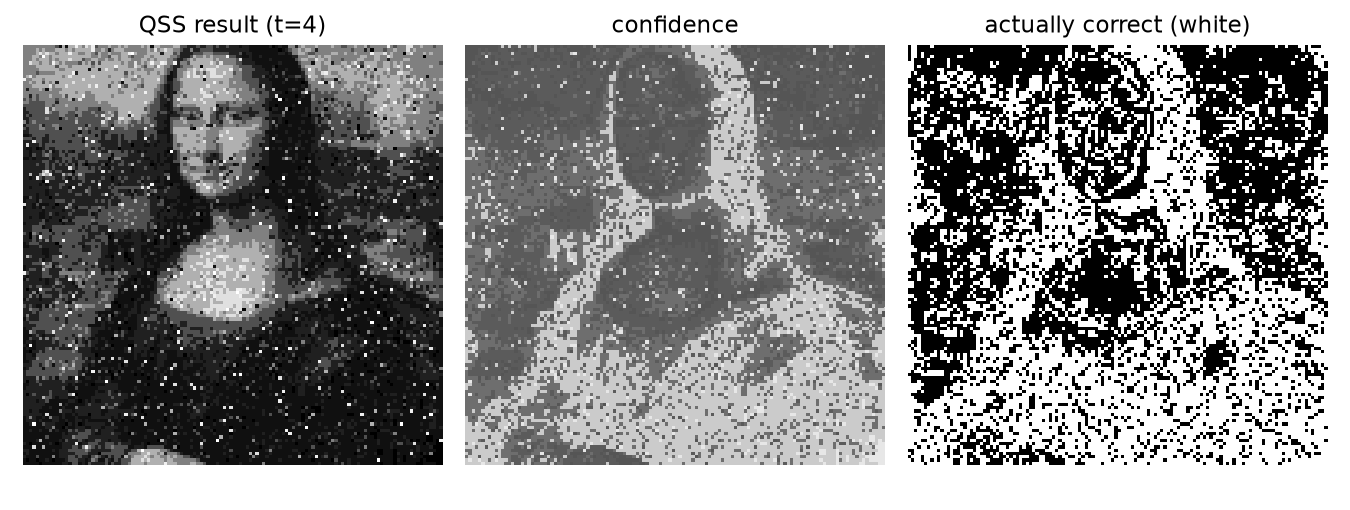
\includegraphics[width=0.75\textwidth]{confidence_t4.png}
\caption{QSS result ($t=4$), its confidence map $c(y)$ from
Eq.~\eqref{eq:conf} (bright $=$ likely correct), and the pixels that are
actually correct (white).}
\label{fig:conf}
\end{figure*}

\begin{figure*}[t]
\centering
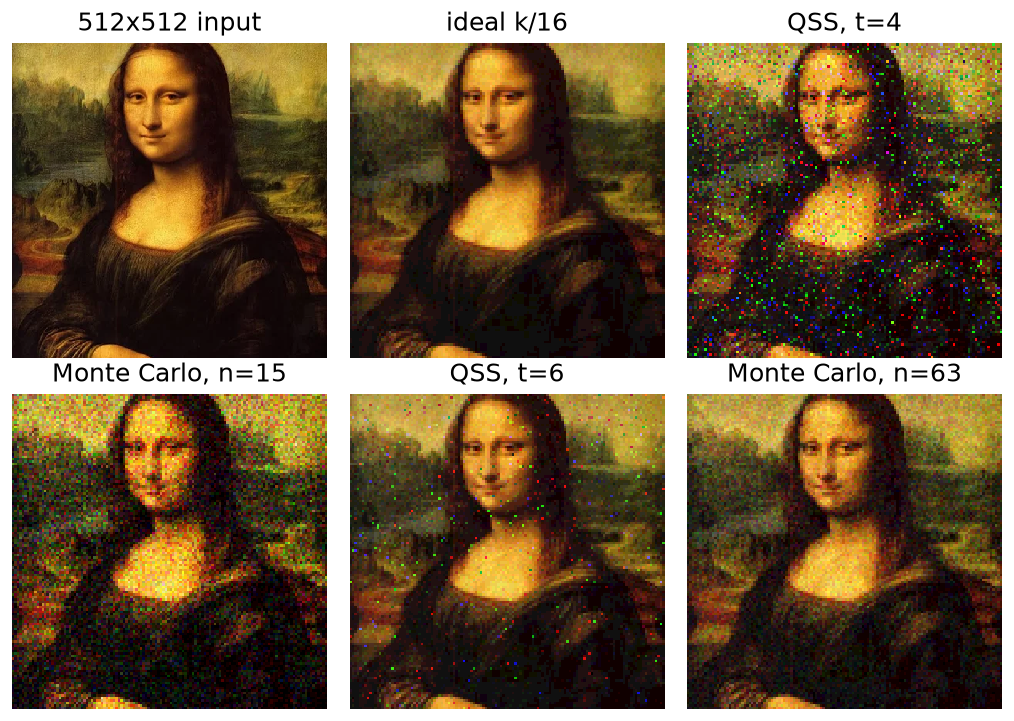
\includegraphics[width=\textwidth]{comparison_rgb.png}
\caption{Colour by bitplanes. From left: $512\times512$ input; ideal; QSS
$t=4$; Monte Carlo $n=15$; QSS $t=6$; Monte Carlo $n=63$.}
\label{fig:rgb}
\end{figure*}

\paragraph{Error level.}
In the book's setting ($t=4$, one readout), QSS lowers the MAE by $21\%$ and
gives $1.78\times$ as many exact pixels. The book reports about $33\%$ and
about $2\times$ for its synthetic test image. At $t=6$ the MAE reduction grows
to $64\%$, and the exact-pixel ratio is $1.67\times$ ($91.1\%$ versus
$54.6\%$). This is qualitatively consistent with the $O(1/N)$ versus
$O(n^{-1/2})$ scaling. Part of the QSS gain from $t=4$ to $t=6$, however, comes
from going from 9 to 17 decodable levels. In addition, the $1/\delta^2$ tails of
the Fej\'er kernel make the single-readout error scale more like
$O(\log N/N)$.

\paragraph{Character of the noise.}
The error maps in Fig.~\ref{fig:gray} show the effect described in the
book. Monte Carlo error is a fine grain on \emph{every} pixel, largest where
$p(1-p)$ is largest, i.e.\ at mid-tones. QSS leaves most pixels exactly right
and puts the rest of its error into fewer but larger mistakes, up to $0.94$
in the worst pixel. At $t=4$ these comprise small offsets for the eight
undecodable mid-tone levels, together with isolated high-contrast specks.
At $t=6$ only $8.9\%$ of pixels are wrong, and these are mostly isolated
specks. A speck appears when a readout lands in the slowly decaying tail of
the Fej\'er kernel, which wraps around modulo $N$. Readouts on the mirror peak
$N-y$ are harmless, because they decode to the same $k$.
In the book's words, conventional supersampling \emph{converges toward} the
exact answer, while QSS raises the \emph{probability} of the exact answer.
Isolated specks are easy to remove afterwards, for example with a median
filter or by re-sampling; a uniform grain is not.

\paragraph{Confidence map.}
Figure~\ref{fig:conf} shows Eq.~\eqref{eq:conf} for $t=4$. It is computed
from the readouts alone, without knowledge of the true image. Confidence is
high for very dark tiles ($y\approx N/2=8$) and very bright tiles
($y\approx0$), and low for mid-tones, where the table columns overlap. The
Pearson (point-biserial) correlation between $c(y)$ and actual correctness is
$0.47$. The map could therefore steer a second pass that re-samples only the
low-confidence pixels.

\paragraph{Colour.}
Following the book's ``Adding Color'' section, the R, G and B bitplanes are
supersampled independently and recombined (Fig.~\ref{fig:rgb}). Each channel
has 17 levels, giving $17^3=4913\approx2^{12.3}$ colours per pixel. This
matches the book's ``effectively 12-bit-per-pixel'' image. Over all channels at
equal cost ($t=4$, $n=15$), QSS has an MAE of $0.050$ with $58.7\%$ exact
values, against $0.064$ and $34.0\%$ for Monte Carlo. At $t=6$, $n=63$ the
figures are $0.0096$ and $92.4\%$ against $0.0285$ and $58.9\%$. A QSS error
shows up as a saturated red, green or blue speck: one bitplane is wrong while
the other two remain exact.

%-------------------------------------------------------------------------
\section{Discussion}\label{sec:disc}

\paragraph{What the QPU contributes.}
The QSS circuit never outputs an individual subpixel value; it estimates
$k=\sum_x f(x)$ over all 16 subpixels in superposition. The shader still
runs $2^t-1$ times per pixel, so there is no speed-up in shader calls. The
benefit is the shape of the error distribution and its faster decrease with
$N$.

\paragraph{Ambiguity at $t=4$.}
The symmetry $P(y\mid k)=P(N-y\mid k)$ leaves only nine distinguishable
outcomes for 17 counts. Moreover, mid-tones are crowded in phase: near
$\theta=\pi/4$ the map $k\mapsto\varphi$ is flattest, and $\varphi_+$ for
$k=8$ and $k=9$ differ by only $0.020<1/N=0.0625$. Both effects explain the
speckle and the low confidence at mid-tones, and both disappear at $t=6$.

\paragraph{Cost of a photographic shader.}
The book's shaders draw shapes with a few arithmetic gates. A photograph has
no such formula, so Eq.~\eqref{eq:oracle} needs up to 16 multi-controlled gates
per oracle call. One tile then needs thousands of CNOT gates, far beyond
today's noisy hardware. Compressing the oracle would reduce this cost, for
example by exclusive-sum-of-products (ESOP) or Reed--Muller synthesis of $f$,
or by flipping the black subpixels together with a global sign when $k>8$.

\paragraph{Other image representations.}
FRQI~\cite{frqi} stores grey levels in a rotation angle, and
NEQR~\cite{neqr} stores them in a basis-state register; both hold greyscale
images without dithering. As the book notes, putting brightness into
amplitudes would break the quantum sum estimation that QSS relies on. I
therefore keep a one-bit phase encoding and obtain tone through dithering and
bitplanes.

\paragraph{Limitations.}
All results come from noiseless simulation, and the bitmap is prepared
classically. The per-tile readouts are sampled from the lookup table, which is
justified by the tests in Table~\ref{tab:verify}. As discussed in the Monte
Carlo baseline subsection, the classical baseline uses a fixed budget. The
results characterise the algorithm; they do not demonstrate a hardware
advantage.

%-------------------------------------------------------------------------
\section{Conclusion}
I drew the Mona Lisa with the complete QSS pipeline of Chapter~11. The
pipeline uses phase-encoded tiles, a lookup-table shader, controlled Grover
iterations, an inverse QFT, a lookup table with the closed form
Eq.~\eqref{eq:lut}, confidence maps and colour bitplanes. At equal sampling
cost, QSS gives a lower mean error than Monte Carlo and nearly twice as many
exactly correct pixels. Its noise is concentrated in fewer, larger mistakes
rather than spread as grain over every pixel. This reproduces the book's
central point: a QPU can be useful by redistributing noise, even without
being faster.

\section*{Code availability}
The code and results are available at
\url{https://github.com/kanaji2002/Quantum-homework-2}.
\texttt{src/prepare\_image.py} prepares the image (Sec.~\ref{sec:prep}).
\texttt{src/qss.py} builds the circuits, runs the verification including
test~(d) and the expected values, and draws all figures; it takes about
80\,s on a laptop. Numerical results are in \texttt{results/metrics.json}.

\begin{thebibliography}{9}\small
\bibitem{pqc} E.~R.~Johnston, N.~Harrigan, M.~Gimeno-Segovia,
\emph{Programming Quantum Computers}, O'Reilly, 2019, Ch.~11.
\bibitem{brassard} G.~Brassard, P.~H{\o}yer, M.~Mosca, A.~Tapp, ``Quantum
amplitude amplification and estimation,'' \emph{Contemp.\ Math.}\
\textbf{305}, 53--74 (2002).
\bibitem{frqi} P.~Q.~Le, F.~Dong, K.~Hirota, ``A flexible representation of
quantum images,'' \emph{Quantum Inf.\ Process.}\ \textbf{10}, 63--84 (2011).
\bibitem{neqr} Y.~Zhang, K.~Lu, Y.~Gao, M.~Wang, ``NEQR: a novel enhanced
quantum representation of digital images,'' \emph{Quantum Inf.\ Process.}\
\textbf{12}, 2833--2860 (2013).
\end{thebibliography}

\end{document}
